%% Manuscript for Chaos (AIP Publishing), REVTeX 4.2, AIP substyle.
%%   * `reprint' gives the two-column reading version;
%%     use `preprint' for submission.
%%   * `article-title' prints article titles in the reference list.
%%   * If only REVTeX 4.1 is available, change revtex4-2 -> revtex4-1 below.
\documentclass[%
  aip,cha,
  amsmath,amssymb,
  reprint,
  floatfix,
  article-title,
]{revtex4-2}

\usepackage[utf8]{inputenc}
\usepackage[T1]{fontenc}
\usepackage{mathptmx}
\usepackage[scaled=0.92]{helvet}
\usepackage{graphicx}
\usepackage{bm}
\usepackage{xcolor}
\usepackage{etoolbox}
\usepackage{float}
\usepackage{algorithm}
\usepackage{algorithmic}
\usepackage[hidelinks]{hyperref}

\renewcommand{\algorithmicrequire}{\textbf{Input:}}
\raggedbottom

%% Placeholder for information that the authors still have to supply.
\newcommand{\AQ}[1]{\textcolor{red}{[#1]}}

%% AIP: the corresponding author's e-mail is set after the affiliations.
\makeatletter
\def\@email#1#2{%
 \endgroup
 \patchcmd{\titleblock@produce}
  {\frontmatter@RRAPformat}
  {\frontmatter@RRAPformat{\produce@RRAP{*#1\href{mailto:#2}{#2}}}\frontmatter@RRAPformat}
  {}{}
}%
\makeatother

\begin{document}

\title[Environment-dependent peer pressure with reinforcement learning]{Environment-dependent peer pressure in spatial public goods games with reinforcement learning}

%% Author block: placeholders
\author{First Author}
\affiliation{Department, Institution, City Postal Code, Country}
\author{Corresponding Author}
\email{corresponding.author@institution.edu}
\affiliation{Department, Institution, City Postal Code, Country}

\date{\today}

\begin{abstract}
Peer pressure is a common form of social influence and affects the evolution of cooperation in social dilemmas. Existing models usually treat peer pressure as a rule that does not change with the local behavioral environment, whereas in reality the behavior that receives pressure depends on what most members of a group do. How such pressure interacts with individual learning remains unclear. To address this, we propose an environment-dependent peer pressure mechanism in a spatial public goods game with reinforcement learning. Defectors receive pressure in groups with enough cooperators, and cooperators receive pressure in the other groups. Individuals update their actions by Q-learning, and their state includes both their own action and the environment of the current group. We find that weak pressure allows cooperation to emerge at lower synergy factors, whereas strong pressure yields higher cooperation levels at higher synergy factors. For a given synergy factor, cooperation increases with the pressure intensity up to an optimal value and then drops abruptly to zero. Under moderate pressure, cooperative clusters survive and individuals learn to cooperate in cooperative environments. Under strong pressure, such environments disappear before this preference can be learned. In addition, the threshold that defines a cooperative environment changes the response of cooperation to pressure, and a state that includes both the action and the environment supports cooperation over a wider range of synergy factors than a state with only one of them. This study shows how local social feedback and individual learning jointly affect the evolution of cooperation.
\end{abstract}

\maketitle

%% Lead Paragraph (required by Chaos)
\begin{quotation}
Social disapproval can change how people behave in groups. However, the behavior that is disapproved of is not always the same. In a group where most members contribute to a common good, those who do not contribute are criticized. In a group where few members contribute, the contributors are the ones who differ from the others. We include this feature in a public goods game on a lattice, where individuals learn from their own experience through reinforcement learning and can tell whether their current group is mostly cooperative. We find that moderate pressure helps clusters of cooperators to survive and expand, so that cooperation finally reaches a high level. When the pressure is too strong, cooperative groups disappear at an early stage and cooperation does not recover. The outcome also depends on how many cooperators are required for a group to be regarded as cooperative and on the information that individuals use for learning.
\end{quotation}

\section{Introduction}\label{sec:intro}

Cooperation is widely observed in biological and social systems, ranging from microbial communities to human societies.\cite{axelrod1981evolution,rand2013human}
However, cooperative behaviors require individuals to bear a cost, while the resulting collective benefits can be exploited by others.\cite{sigmund2010calculus}
Understanding how cooperation can emerge and persist despite the advantage of selfish behaviors has therefore become a central topic in many disciplines.\cite{pennisi2005did}

Evolutionary game theory provides a framework for investigating this problem.\cite{smith1973logic,taylor1978evolutionary,nowak2006evolutionary}
Among various models, the public goods game (PGG) is widely used to describe social dilemmas in which individuals decide whether to contribute to a common pool.\cite{hauert2006evolutionary,szolnoki2016competition,zhu2024stochastic}
Spatial PGGs further include population structure and local interactions, which allow cooperators to form clusters and resist exploitation.\cite{nowak1992evolutionary,ohtsuki2006simple,szabo2007evolutionary,szolnoki2009impact,perc2013evolutionary,perc2017statistical,zhu2025multilayer}
On this basis, many mechanisms that support cooperation have been studied,\cite{perc2010coevolutionary} including punishment,\cite{fehr2002altruistic,helbing2010punish,chen2014probabilistic,szolnoki2017antisocial,xie2024regulation} reward,\cite{rand2009positive,szolnoki2010reward} reputation,\cite{milinski2002helps,zhu2024synergy} and environmental feedback.\cite{weitz2016oscillating,tilman2020evolutionary,wang2020eco,hu2025dynamic}

Peer pressure is another mechanism that influences cooperation and other collective behaviors.\cite{szolnoki2015conformity,xu2026synergistic}
Individuals whose behavior differs from that of the people around them may face disapproval or exclusion, and they tend to adjust their behavior accordingly.\cite{asch1952social,cialdini1990focus}
In evolutionary games, peer pressure has been modeled in two ways.
In the first, each individual is penalized in proportion to the number of its neighbors that hold the opposite strategy, whether it cooperates or defects.\cite{yang2015peer,hu2021peer,gao2023impact,ma2025evolution}
In the second, cooperation is regarded as the social norm, and only defectors are penalized, in proportion to the number of cooperators in their group.\cite{deng2018peer}
Both rules can promote cooperation, and under the first rule a moderate pressure intensity is the most effective.\cite{yang2015peer,gao2023impact}

In both rules, the behavior that receives pressure is specified in advance and is the same in every group.
In reality, however, what a group expects of its members is largely determined by what most of them do.
In a team where most members work hard, a member who contributes little is criticized.
In a team where most members contribute little, a member who works hard may instead be resented, because this effort raises what is expected of the others.
Public goods experiments have indeed found that punishment is directed at high contributors as well as at free riders.\cite{herrmann2008antisocial}
The prevailing behavior of a group thus acts as a local environment, which determines the behavior that receives pressure and is in turn changed by the actions of the group members.
Neither rule describes this situation.
Under the first rule, both behaviors are penalized in every mixed group, including the behavior of the majority.
Under the second rule, cooperators are never penalized, even when almost all members of their group defect.

In addition, strategies in these models spread by imitation,\cite{szabo2007evolutionary,traulsen2010human} and each individual uses one strategy in all its interactions.
When the pressure depends on the group, however, an individual that belongs to several groups may be expected to behave differently in each of them.
Reinforcement learning describes individuals who choose actions according to their current state and adjust these choices according to the rewards received.\cite{young2009learning,sutton2018reinforcement,xie2026reinforcement,zheng2026brief}
In particular, Q-learning\cite{watkins1992qlearning} has been applied to PGGs and other social dilemmas,\cite{zheng2024evolution,shi2024model,wang2025spatial,mintz2025evolutionary,li2025cooperation} also in combination with punishment, reward, and reputation.\cite{zhao2024emergence,wang2023synergistic,ren2024interaction,shen2024adaptive,li2026reputation}
In most of these studies, however, the state of an individual is its own previous action,\cite{wang2022levy,fan2022incorporating,du2026shaping} and the behavior of its group is not included.
Recent studies have shown that information about the environment affects cooperation,\cite{kleshnina2023effect,lv2025reinforcement,li2025environmental} but it has not been combined with peer pressure that depends on this environment.

In this work, we propose an environment-dependent peer pressure mechanism in a spatial PGG with Q-learning.
A group is a cooperative environment if its number of cooperators reaches a threshold, and a defective environment otherwise.
Defectors receive pressure in cooperative environments, and cooperators receive pressure in defective environments.
The state of each individual consists of its own action and the environment of its current group, so that it can learn different actions for different environments.
The rule that penalizes only defectors is recovered at the lowest threshold, and the rule that penalizes both behaviors is used for comparison.
We find that weak pressure allows cooperation to emerge at lower synergy factors, whereas strong pressure yields higher cooperation levels at higher synergy factors, and that cooperation collapses once the pressure exceeds an optimal intensity.
Spatial patterns and learning dynamics show that this collapse occurs because strong pressure removes cooperative environments before individuals learn to cooperate in them.
The threshold further changes the response of cooperation to pressure.


\section{Model}\label{sec:model}

\subsection{Spatial public goods game}\label{sec:pgg}

We consider a spatial public goods game on a square lattice with periodic boundary conditions. The population consists of $L\times L$ individuals, with each individual occupying a single lattice site. Each interaction group consists of a focal individual and its four nearest neighbors, so that the group size is $g=5$. Each individual therefore belongs to five overlapping groups, including the group centered on itself and the groups centered on its four neighbors.

Each individual $i$ adopts one of two actions, $a_i\in\mathcal{A}=\{\mathrm{C},\mathrm{D}\}$, where $\mathrm{C}$ denotes cooperation and $\mathrm{D}$ denotes defection. In each group interaction, cooperators contribute a fixed cost $c=1$, whereas defectors contribute nothing. The total contribution is multiplied by the synergy factor $r$ and equally distributed among all group members. The payoff of individual $i$ in a group interaction is
\begin{equation}
\pi_i=\frac{r\,n_{\mathrm{C}}}{g}-c_i,
\label{eq:payoff}
\end{equation}
where $n_{\mathrm{C}}$ is the number of cooperators in the group, and $c_i=1$ if individual $i$ cooperates and $c_i=0$ otherwise.

\subsection{Environment-dependent peer pressure}\label{sec:pressure}

We assume that peer pressure depends on the local environment of each interaction group. The environment is determined separately for each group according to the environmental threshold $T$, which is an integer between $0$ and $g$. When the number of cooperators in the group satisfies $n_{\mathrm{C}}\geq T$, the group is in a cooperative environment, denoted by $\mathrm{G}$. Otherwise, it is in a defective environment, denoted by $\mathrm{B}$.

The environment determines which behavior receives pressure. In a cooperative environment, defectors receive pressure from the cooperators in the group. In a defective environment, cooperators receive pressure from the defectors in the group. The peer pressure on individual $i$ is defined as
\begin{equation}
P_i=
\begin{cases}
-\beta\,n_{\mathrm{C}}, & a_i=\mathrm{D},\ n_{\mathrm{C}}\geq T,\\
-\beta\,n_{\mathrm{D}}, & a_i=\mathrm{C},\ n_{\mathrm{C}}<T,\\
0, & \text{otherwise},
\end{cases}
\label{eq:pressure}
\end{equation}
where $n_{\mathrm{D}}=g-n_{\mathrm{C}}$ is the number of defectors in the group and $\beta$ is the intensity of peer pressure. Here, $a_i$ and $n_{\mathrm{C}}$ refer to the actions implemented in the current interaction. The effective reward of individual $i$ in a group interaction is
\begin{equation}
R_i=\pi_i+P_i.
\label{eq:effective}
\end{equation}

Figure~\ref{fig:Fig1} illustrates these definitions for two overlapping groups and $T=3$, which for $g=5$ corresponds to the simple-majority rule. Two limiting cases are worth noting. For $T\leq1$, a group can be defective only if it contains no cooperator, so cooperators are never pressured. The cases $T=0$ and $T=1$ then differ only in whether a fully defecting group is distinguished as a separate environment. For $T=g$, a group is cooperative only if it contains no defector, so defectors are never pressured.

\begin{figure}[t]
\centering
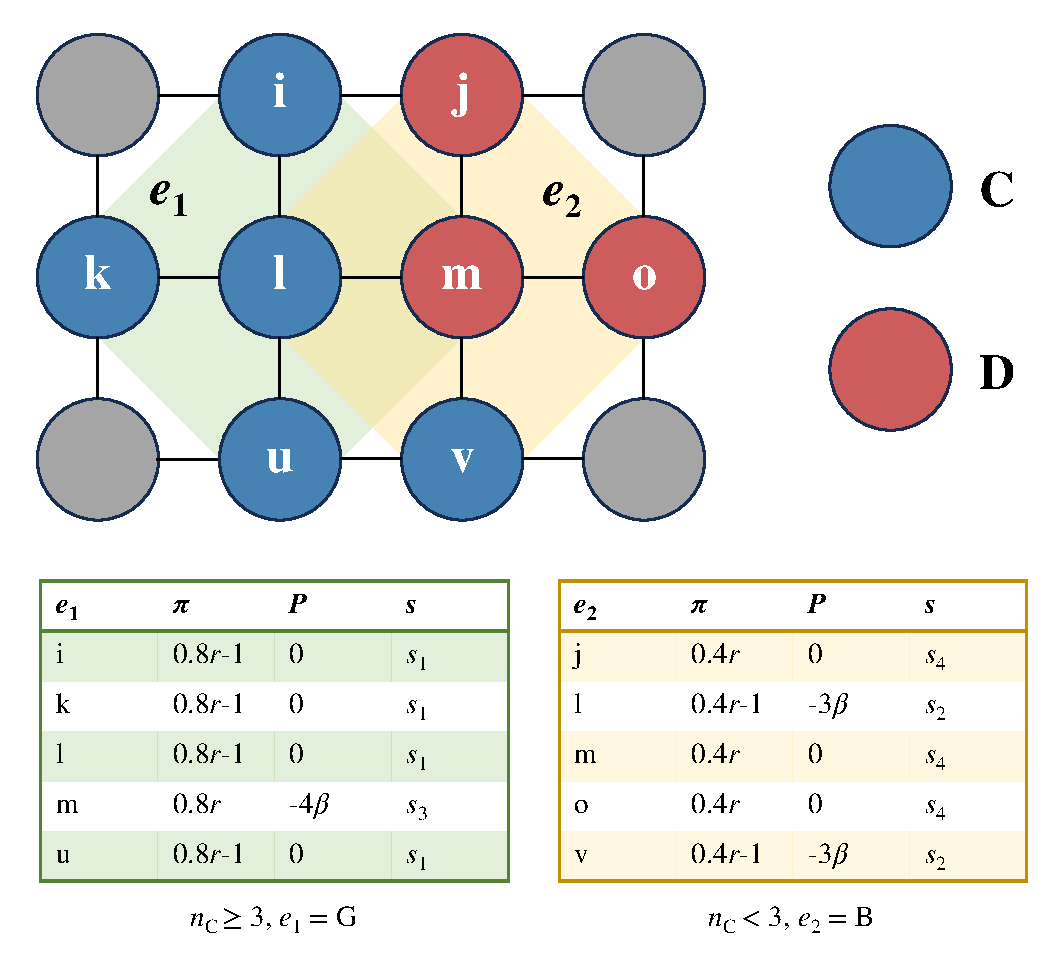
\includegraphics[width=\linewidth]{Fig_1.pdf}
\caption{
The environment of a group determines the payoff, peer pressure, and state of its members. Two overlapping interaction groups are shown for $T=3$. Blue and red circles denote cooperators and defectors, and gray circles are individuals outside the two groups. Group $e_1$, centered on $l$, contains four cooperators and is a cooperative environment ($\mathrm{G}$), so its defector $m$ receives pressure. Group $e_2$, centered on $m$, contains two cooperators and is a defective environment ($\mathrm{B}$), so its cooperators $l$ and $v$ receive pressure. The tables list the payoff $\pi$, the peer pressure $P$, and the state $s$ of each group member. Individuals $l$ and $m$ belong to both groups and have different states in them.
}
\label{fig:Fig1}
\end{figure}

\subsection{Q-learning with environmental information}\label{sec:qlearning}

To describe how individuals adapt their behavior, we introduce Q-learning\cite{watkins1992qlearning,sutton2018reinforcement} into the spatial public goods game. Previous studies have often used the previous action of an individual to define its state.\cite{wang2022levy,fan2022incorporating,du2026shaping} However, including environmental information in the state allows individuals to distinguish group environments during learning.\cite{li2025environmental} In our model, the effective reward depends on both the action of an individual and the environment of the group. The state is therefore defined by the current action of the individual and the environment of the interaction group. Combining these two components gives four states, $s_1=(\mathrm{C},\mathrm{G})$, $s_2=(\mathrm{C},\mathrm{B})$, $s_3=(\mathrm{D},\mathrm{G})$, and $s_4=(\mathrm{D},\mathrm{B})$.

For each individual, the Q-table records the expected discounted cumulative reward of each state-action pair and has the form
\begin{equation}
Q_i=
\begin{bmatrix}
Q_i(s_1,\mathrm{C})&Q_i(s_1,\mathrm{D})\\
Q_i(s_2,\mathrm{C})&Q_i(s_2,\mathrm{D})\\
Q_i(s_3,\mathrm{C})&Q_i(s_3,\mathrm{D})\\
Q_i(s_4,\mathrm{C})&Q_i(s_4,\mathrm{D})
\end{bmatrix},
\label{eq:qtable}
\end{equation}
where the two columns correspond to the two actions. Because the environment is defined for each group, the same individual is generally in different states in the different groups to which it belongs (see individuals $l$ and $m$ in Fig.~\ref{fig:Fig1}), but it uses a single Q-table in all of them.

In state $s$, an individual selects its action according to the $\epsilon$-greedy rule. With probability $1-\epsilon$ it chooses the action with the higher Q-value in the current state, and with probability $\epsilon$ it chooses one of the two actions at random. When the two Q-values are equal, one action is selected at random. After all members of the group have implemented their actions, individual $i$ receives the effective reward $R_i$ and updates its Q-table according to
\begin{equation}
Q_i(s,a)\leftarrow(1-\alpha)\,Q_i(s,a)+\alpha\Bigl[R_i+\gamma\max_{a'\in\mathcal{A}}Q_i(s',a')\Bigr],
\label{eq:q-learning}
\end{equation}
where $\alpha$ is the learning rate and $\gamma$ is the discount factor. The new state $s'$ is determined by the action just implemented and the environment of the same group after all its members have acted.

\subsection{Simulation procedure}\label{sec:simulation}

Initially, each individual is assigned $\mathrm{C}$ or $\mathrm{D}$ with equal probability, and all Q-values are set to zero. We use a single group interaction as the elementary unit of learning, rather than accumulating payoffs over all overlapping groups.\cite{li2025environmental} In each elementary step, a focal individual is randomly selected, and the group centered on it plays the game once. All members of this group select their actions, receive their effective rewards, and update their Q-tables according to the environment of this group. One Monte Carlo step (MCS) consists of $L^2$ elementary steps, so that each individual participates in $g$ group interactions on average. The complete procedure is summarized in Algorithm~\ref{alg:PGG_Qlearning}.

\begin{algorithm}[H]
\caption{Spatial public goods game with peer pressure and Q-learning.}
\label{alg:PGG_Qlearning}
\begin{algorithmic}[1]
\REQUIRE $L$, $r$, $T$, $\beta$, $\alpha$, $\gamma$, $\epsilon$, and the number of Monte Carlo steps $t_{\max}$
\FOR{each individual $i$}
    \STATE Set $a_i$ to $\mathrm{C}$ or $\mathrm{D}$ with equal probability;
    \STATE Set $Q_i(s,a)=0$ for all $s$ and $a$;
\ENDFOR
\FOR{$t=1$ to $t_{\max}$}
    \FOR{$n=1$ to $L^2$}
        \STATE Randomly select a focal individual; let $\Omega$ be the group formed by it and its four nearest neighbors;
        \STATE Determine the environment $e$ of $\Omega$;
        \FOR{each individual $j\in\Omega$}
            \STATE $s_j\leftarrow(a_j,e)$;
            \STATE With probability $\epsilon$, select $a'_j$ randomly from $\mathcal{A}$; otherwise select the action $a'_j$ with the higher Q-value in state $s_j$ (randomly if the two values are equal);
        \ENDFOR
        \STATE Implement all actions simultaneously, $a_j\leftarrow a'_j$ for all $j\in\Omega$;
        \STATE Determine the new environment $e'$ of $\Omega$;
        \FOR{each individual $j\in\Omega$}
            \STATE Calculate $\pi_j$, $P_j$, and $R_j$ by Eqs.~\eqref{eq:payoff}--\eqref{eq:effective};
            \STATE $s'_j\leftarrow(a_j,e')$;
            \STATE Update $Q_j(s_j,a_j)$ by Eq.~\eqref{eq:q-learning};
        \ENDFOR
    \ENDFOR
\ENDFOR
\end{algorithmic}
\end{algorithm}

The cooperation level $\rho_{\mathrm{C}}$ is the fraction of cooperators in the population. Its stationary value is calculated by averaging over the last $10^5$ MCS of a simulation lasting $10^6$ MCS. For parameter sets that do not reach a stationary state within $10^6$ MCS, the simulation is extended to $10^8$ MCS, and the average is taken over the last $10^7$ MCS. Each data point is averaged over 20 independent runs. Unless stated otherwise, we use $L=100$, $T=3$, and the learning parameters $\alpha=0.1$, $\gamma=0.9$, and $\epsilon=0.01$.\cite{zhao2024emergence,zheng2024evolution,li2025environmental}


\section{Results and discussion}\label{sec:results}

\subsection{Interplay of pressure intensity and synergy factor}\label{sec:res-r-beta}

\begin{figure*}[t]
\centering
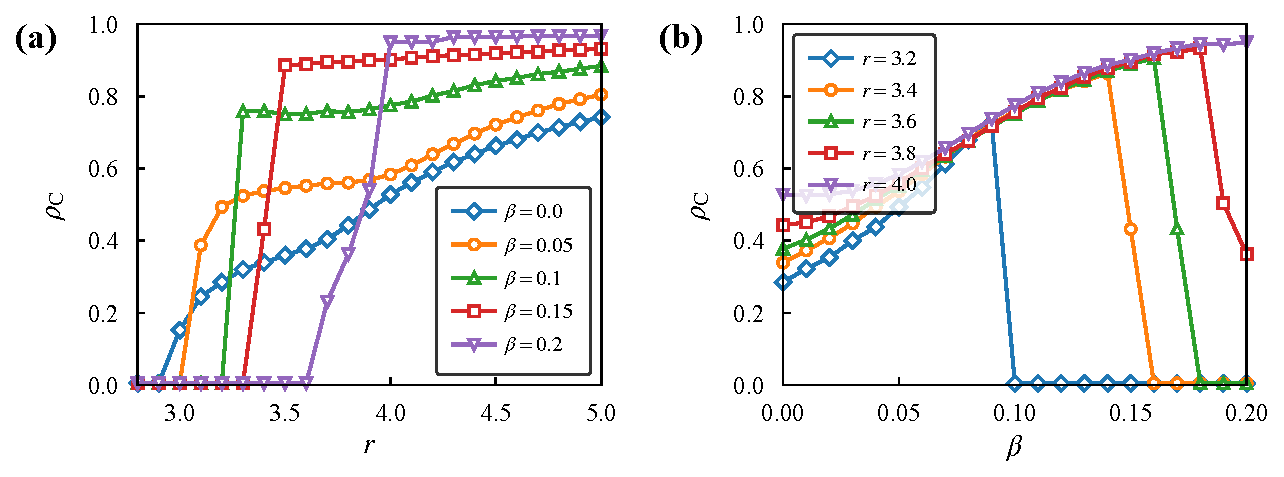
\includegraphics[width=\linewidth]{Fig_2.pdf}
\caption{
Weak pressure favors the emergence of cooperation at small synergy factors, whereas strong pressure yields higher cooperation at large synergy factors. (a) Cooperation level $\rho_{\mathrm{C}}$ as a function of the synergy factor $r$ for different pressure intensities $\beta$. (b) $\rho_{\mathrm{C}}$ as a function of $\beta$ for different values of $r$. For $r<4$, $\rho_{\mathrm{C}}$ reaches its maximum at an optimal $\beta$ and then drops abruptly to zero.
}
\label{fig:Fig2}
\end{figure*}

We first investigate how peer pressure affects cooperation under different synergy factors. Figure~\ref{fig:Fig2}(a) shows the cooperation level $\rho_{\mathrm{C}}$ as a function of $r$ for different values of $\beta$. Without pressure, cooperation emerges at the lowest synergy factor and increases gradually with $r$. As $\beta$ increases, the onset of cooperation shifts toward higher $r$. When $r$ is small, a smaller $\beta$ therefore makes cooperation more likely to emerge. Once cooperation has emerged, however, a larger $\beta$ produces a higher cooperation level, and the order of the curves at large $r$ is the reverse of the order of their onsets. Weak pressure and strong pressure are thus each more favorable in a different range of $r$. In addition, the emergence of cooperation becomes sharper as $\beta$ increases. The cooperation level rises gradually from zero for $\beta=0$, whereas for larger $\beta$ it jumps from zero to a high value within a narrow range of $r$.

Figure~\ref{fig:Fig2}(b) shows $\rho_{\mathrm{C}}$ as a function of $\beta$ for different values of $r$. For each $r$, the cooperation level first increases with $\beta$. As $\beta$ increases, the curves for different $r$ approach each other, which indicates that the cooperation level is mainly determined by $\beta$ as long as cooperation is maintained. For $r<4$, there is an optimal $\beta$ that maximizes cooperation. Beyond this value, cooperation collapses abruptly to zero, in a manner similar to a discontinuous phase transition.\cite{perc2017statistical} Both the optimal $\beta$ and the collapse shift toward larger $\beta$ as $r$ increases. For $r=4.0$, cooperation is maintained up to the largest $\beta$ examined.

These observations can be understood from the difference between the effective rewards of cooperation and defection in a single interaction, which is derived in the Appendix. According to Eq.~\eqref{eq:delta}, peer pressure raises the reward of cooperation relative to defection in groups where most co-players cooperate, and lowers it in groups where most co-players defect. Pressure therefore strengthens the behavior of the local majority. When $r$ is small, the cost of cooperation is high and defectors more easily become the local majority, so that stronger pressure suppresses cooperation. When $r$ is large, cooperative groups are easier to maintain, and stronger pressure on the defectors in these groups raises the cooperation level. The same reasoning explains why a larger $r$ allows cooperation to persist under stronger pressure.

\subsection{Time evolution and spatial patterns}\label{sec:res-time}

\begin{figure*}[t]
\centering
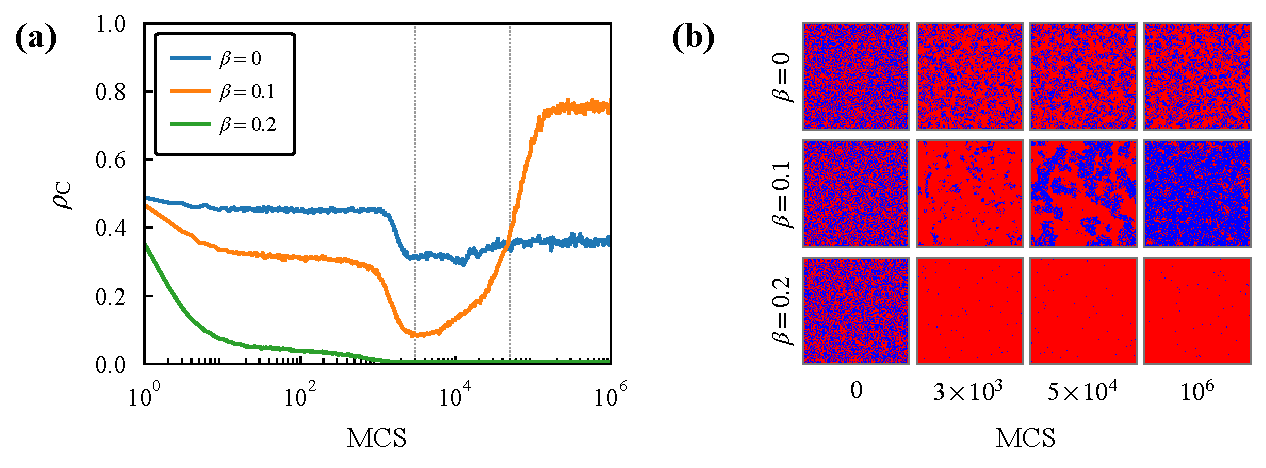
\includegraphics[width=\linewidth]{Fig_3.pdf}
\caption{
Moderate pressure allows cooperative clusters to survive and expand, whereas strong pressure leads to defection. (a) Time evolution of the cooperation level $\rho_{\mathrm{C}}$ for $\beta=0$, $0.1$, and $0.2$. The vertical dotted lines mark the times of the second and third snapshots. (b) Spatial snapshots at $0$, $3\times10^{3}$, $5\times10^{4}$, and $10^{6}$~MCS (from left to right) for $\beta=0$, $0.1$, and $0.2$ (from top to bottom). Cooperators and defectors are shown in blue and red, respectively. For each $\beta$, the curve and the snapshots are obtained from the same simulation. The synergy factor is $r=3.5$.
}
\label{fig:Fig3}
\end{figure*}

Figure~\ref{fig:Fig3} presents the time evolution of cooperation and the corresponding spatial patterns at $r=3.5$, comparing the cases without pressure ($\beta=0$), with moderate pressure ($\beta=0.1$), and with strong pressure ($\beta=0.2$).

As shown in Fig.~\ref{fig:Fig3}(a), cooperation initially decreases in all three cases, and stronger pressure produces a faster decline. Without pressure, cooperation shows only a limited recovery after the decline. At $\beta=0.1$, cooperation reaches a lower minimum than without pressure but subsequently recovers to a higher level. At $\beta=0.2$, cooperation rapidly approaches zero and does not recover. Moderate pressure therefore lowers cooperation at the early stage but raises it in the stationary state, whereas strong pressure drives the population toward defection.

Figure~\ref{fig:Fig3}(b) shows the spatial patterns that accompany these trajectories. At $\beta=0.1$, small cooperative clusters survive the initial decline, then expand, and finally occupy most of the lattice. At $5\times10^{4}$~MCS, the cooperation levels at $\beta=0$ and $\beta=0.1$ are comparable. However, cooperators and defectors remain finely mixed without pressure, whereas individuals with the same action form large clusters at $\beta=0.1$. Under strong pressure, the lattice is already dominated by defectors at $3\times10^{3}$~MCS, and only a few isolated cooperators appear later because of exploration. Moderate pressure thus favors the survival and expansion of cooperative clusters, which provides a spatial basis for the recovery of cooperation. Strong pressure removes cooperators before such clusters can form.

\subsection{Learning dynamics under moderate and strong pressure}\label{sec:res-learning}

\begin{figure*}[t]
\centering
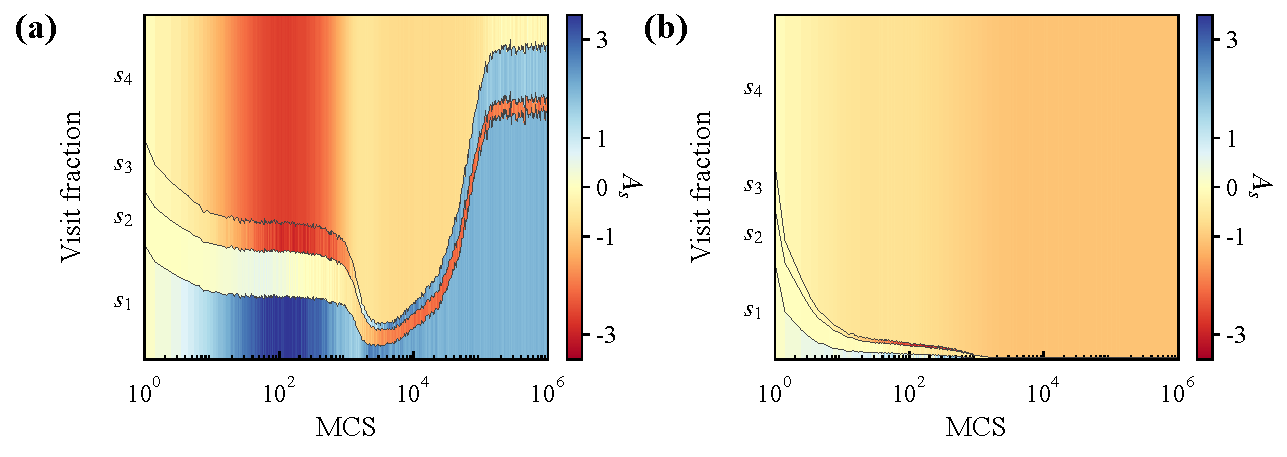
\includegraphics[width=\linewidth]{Fig_4.pdf}
\caption{
Cooperative environments continue to be visited under moderate pressure but disappear under strong pressure. (a) $\beta=0.1$. (b) $\beta=0.2$. The four bands from bottom to top correspond to the states $s_1$, $s_2$, $s_3$, and $s_4$, and the width of each band gives the fraction of visits to that state. The color represents the Q-value difference $A_s$ defined in Eq.~\eqref{eq:gap}, where blue and red indicate a preference for cooperation and defection, respectively. The color scale is nonlinear. The synergy factor is $r=3.5$.
}
\label{fig:Fig4}
\end{figure*}

To further understand why moderate pressure promotes cooperation and strong pressure suppresses it, Fig.~\ref{fig:Fig4} examines how often each state is visited and which action is preferred in it. The preference is measured by the Q-value difference
\begin{equation}
A_s(t)=\bigl\langle Q_i(s,\mathrm{C})-Q_i(s,\mathrm{D})\bigr\rangle_{s,t},
\label{eq:gap}
\end{equation}
where $\langle\cdot\rangle_{s,t}$ denotes the average over all visits to state $s$ during MCS $t$. Q-values are evaluated before the corresponding updates, and repeated visits by the same individual are counted separately. Positive and negative values of $A_s$ indicate an average preference for cooperation and defection, respectively.

Under moderate pressure, Fig.~\ref{fig:Fig4}(a) shows that $A_{s_1}$ increases rapidly during the early stage, while $A_{s_3}$ is first negative and later becomes positive. Cooperation thus becomes preferred, on average, in both states associated with cooperative environments. Although the overall cooperation level initially declines, $s_1$ and $s_3$ continue to be visited, because the surviving cooperative clusters shown in Fig.~\ref{fig:Fig3} keep providing cooperative environments. In these environments, defectors receive pressure while cooperators do not. These interactions allow individuals to gradually develop a preference for cooperation, including in $s_3$, where their current action is defection. In the stationary state, $A_{s_2}$ is negative and $A_{s_4}$ remains slightly negative, so that defection is preferred in defective environments. Individuals have thus learned to cooperate in cooperative environments and to defect in defective ones. The persistence of cooperative environments therefore retains the learning opportunities that support the recovery of cooperation.

Under strong pressure, Fig.~\ref{fig:Fig4}(b) shows a rapid concentration of visits in $s_4$, which combines defection with a defective environment. With Q-values initially set to zero, the earliest updates are driven mainly by immediate rewards. Stronger pressure on cooperators in defective environments favors the early development of a preference for defection, which contributes to the faster decline of cooperation. Visits to $s_1$ and $s_3$ consequently become rare, leaving almost no opportunities for learning in cooperative environments. Meanwhile, $A_{s_4}$ remains negative, indicating a persistent preference for defection. It should be noted that strong pressure does not reduce the reward of cooperation in cooperative environments, as shown by Eq.~\eqref{eq:delta}. Instead, it accelerates the loss of these environments, which limits the development of a preference for cooperation and prevents the recovery of cooperation.

\subsection{Role of the environmental threshold}\label{sec:res-threshold}

\begin{figure*}[t]
\centering
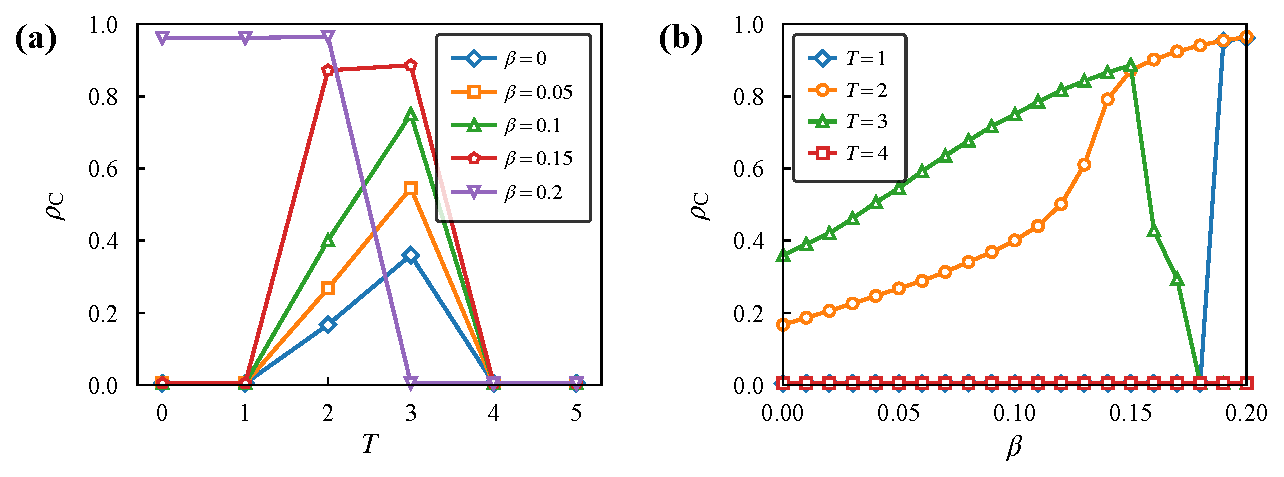
\includegraphics[width=\linewidth]{Fig_5.pdf}
\caption{
The environmental threshold changes the response of cooperation to peer pressure. (a) Cooperation level $\rho_{\mathrm{C}}$ as a function of the environmental threshold $T$ for different pressure intensities $\beta$. (b) $\rho_{\mathrm{C}}$ as a function of $\beta$ for $T=1$, $2$, $3$, and $4$. The synergy factor is $r=3.5$.
}
\label{fig:Fig5}
\end{figure*}

We next examine how the environmental threshold $T$ affects cooperation at $r=3.5$. Figure~\ref{fig:Fig5}(a) shows that cooperation is highest at $T=3$, followed by $T=2$, under weak and moderate pressure. At $\beta=0.2$, high cooperation occurs at $T=0$, $T=1$, and $T=2$, whereas cooperation at $T=3$ is close to zero. At $T=4$ and $T=5$, cooperation remains close to zero for all pressure intensities shown. Thus, intermediate thresholds favor cooperation under weak and moderate pressure, whereas lower thresholds are more favorable under strong pressure. The cooperation level also differs among thresholds at $\beta=0$. Since the rewards do not depend on $T$ in this case, this difference comes from the state definition alone, because $T$ determines how individuals distinguish the two environments during learning.

Figure~\ref{fig:Fig5}(b) shows how cooperation responds to pressure at each threshold. At $T=1$, cooperation remains close to zero over most of the range and rises abruptly only when $\beta$ is close to the largest value examined. Cooperators are always exempt from pressure at this threshold, but defectors face only weak pressure when cooperators are scarce. Only sufficiently strong pressure can constrain defection and enable cooperation to emerge. At $T=2$, cooperation increases monotonically with $\beta$. Only two cooperators are needed to form a cooperative environment, so a cooperator receives pressure only when it is the single cooperator in its group. Stronger pressure then mainly increases the cost of defection and favors cooperation. At $T=3$, cooperation first increases with $\beta$ and then collapses, as analyzed in Secs.~\ref{sec:res-r-beta}--\ref{sec:res-learning}. At $T=4$, cooperation remains close to zero. A cooperative environment requires at least four cooperators, so cooperators receive pressure in most mixed groups and cooperation is difficult to sustain. These results show that the threshold changes both the pressure needed to promote cooperation and the extent to which cooperation can withstand stronger pressure.

\subsection{Comparison of pressure rules and state representations}\label{sec:res-comparison}

\begin{figure*}[t]
\centering
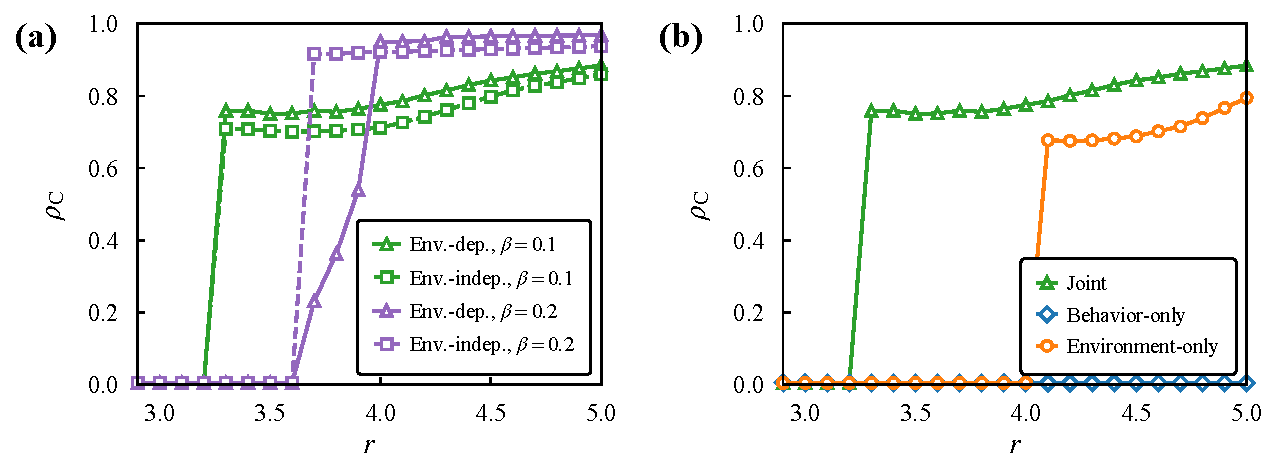
\includegraphics[width=\linewidth]{Fig_6.pdf}
\caption{
Neither pressure rule is better in all cases, and the joint state representation supports cooperation over the widest range of synergy factors. (a) Cooperation level $\rho_{\mathrm{C}}$ as a function of $r$ under environment-dependent pressure (solid lines) and environment-independent pressure (dashed lines) for $\beta=0.1$ and $\beta=0.2$. Both rules use the joint state representation. (b) $\rho_{\mathrm{C}}$ as a function of $r$ for the joint, behavior-only, and environment-only state representations under environment-dependent pressure at $\beta=0.1$.
}
\label{fig:Fig6}
\end{figure*}

To examine the roles of the pressure rule and of the information available for learning, we compare two pressure rules and three state representations. The action set and the learning parameters remain unchanged in these comparisons.

Figure~\ref{fig:Fig6}(a) compares the environment-dependent rule of Eq.~\eqref{eq:pressure} with an environment-independent rule, under which individuals receive pressure from all group members with the opposite action regardless of the group environment,
\begin{equation}
P_i^{\mathrm{ind}}=
\begin{cases}
-\beta\,n_{\mathrm{D}}, & a_i=\mathrm{C},\\
-\beta\,n_{\mathrm{C}}, & a_i=\mathrm{D}.
\end{cases}
\label{eq:indep}
\end{equation}
Both rules use the same four states, so that only the reward differs. At $\beta=0.1$, the two rules give the same onset of cooperation, and the environment-dependent rule yields a slightly higher cooperation level. At $\beta=0.2$, cooperation emerges at a lower $r$ under the environment-independent rule, whereas the environment-dependent rule yields a slightly higher cooperation level at larger $r$. The environment-dependent rule is therefore not better in all cases.

This result can be explained by the reward difference in a single interaction. Suppose that $k$ of the $g-1$ co-players of a focal individual cooperate. Under the environment-independent rule, the effective reward of cooperation minus that of defection is
\begin{equation}
\Delta_k^{\mathrm{ind}}=\frac{r}{g}-1+\beta\,(2k-g+1),
\label{eq:delta-indep}
\end{equation}
because changing the action removes the pressure from one side and adds the pressure from the other side. For $g=5$ and $T=3$, Eqs.~\eqref{eq:delta} and \eqref{eq:delta-indep} are identical for $k=0$, $2$, and $4$. They differ for $k=1$ and $k=3$, where the pressure term is $\mp3\beta$ under the environment-dependent rule and $\mp2\beta$ under the environment-independent rule. The environment-dependent rule therefore gives a stronger incentive to follow the local majority. This raises cooperation where cooperative groups are common and lowers it where they are rare, which is consistent with Fig.~\ref{fig:Fig6}(a).

Figure~\ref{fig:Fig6}(b) compares the three state representations at $\beta=0.1$. With behavior-only states, cooperation remains close to zero throughout the examined range of $r$. With environment-only states, cooperation appears only at large $r$. The joint representation supports cooperation at lower $r$ and yields higher cooperation levels. The behavior-only representation retains the two states $\mathrm{C}$ and $\mathrm{D}$ but omits the group environment, whereas the environment-only representation retains $\mathrm{G}$ and $\mathrm{B}$ but omits the action of the individual. Under the present pressure rule, the reward of an action depends on the environment, so individuals without environmental information cannot learn different actions for different environments. Retaining both types of information allows individuals to learn action values separately for each combination of action and environment. These results show that distinguishing both the individual action and the group environment during learning helps sustain cooperation over a broader range of synergy factors.


\section{Conclusion}\label{sec:conclusion}

Peer pressure is an important form of social influence on cooperation.\cite{yang2015peer,deng2018peer,gao2023impact,ma2025evolution} In previous models, the pressure rule does not change with the local behavioral environment, and how such pressure interacts with individual learning\cite{xie2026reinforcement,zheng2026brief} has remained unclear. In this work, we have proposed an environment-dependent peer pressure mechanism in a spatial public goods game with Q-learning. Defectors receive pressure in groups with enough cooperators, and cooperators receive pressure in the other groups. The state of each individual includes both its own action and the environment of its current group, so that individuals can learn different actions for different environments.

Our results reveal several findings. First, the effect of peer pressure depends on its intensity and on the synergy factor. Weak pressure allows cooperation to emerge at lower synergy factors, whereas strong pressure yields higher cooperation levels at higher synergy factors. For a given synergy factor, there is an optimal pressure intensity, beyond which cooperation collapses abruptly. Higher synergy factors allow cooperation to persist under stronger pressure. Second, the spatial patterns and the learning dynamics explain these results. Under moderate pressure, cooperative clusters survive the initial decline, and individuals learn to cooperate in cooperative environments. Under strong pressure, cooperative environments are lost at the early stage, which restricts the opportunities for learning a preference for cooperation. Third, the environmental threshold changes the response of cooperation to pressure. Intermediate thresholds favor cooperation under weak and moderate pressure, whereas lower thresholds are more favorable under strong pressure. Finally, the environment-dependent rule is not always better than the environment-independent rule, and the joint state representation supports cooperation over a wider range of synergy factors than the behavior-only or the environment-only representation.

These findings show that the effect of peer pressure on cooperation is determined jointly by the pressure rule, the local environment, and the learning process of individuals. The present results are obtained on a square lattice with fixed learning parameters and random initial conditions. Future studies could consider more complex network structures,\cite{shi2024model,zhu2025multilayer} alternative state-transition rules,\cite{guo2022effect} and separate thresholds for the pressure rule and for the state definition.


\begin{acknowledgments}
\AQ{Acknowledgments to be added.}
\end{acknowledgments}

\section*{Author Declarations}

\subsection*{Conflict of Interest}
The authors have no conflicts to disclose.

\subsection*{Author Contributions}
\AQ{Author contributions to be added.}

\section*{Data Availability}
The data that support the findings of this study are available from the corresponding author upon reasonable request.

\appendix*
\section{Reward difference in a single interaction}\label{sec:appendix}

Here we compare the effective rewards of cooperation and defection in a single group interaction. Consider a focal individual and suppose that $k$ of its $g-1$ co-players cooperate, where $k=0,1,\dots,g-1$. From Eqs.~\eqref{eq:payoff}--\eqref{eq:effective}, the effective reward of cooperation minus that of defection is
\begin{equation}
\Delta_k=
\begin{cases}
\dfrac{r}{g}-1+\beta k, & k\geq T,\\[1.5ex]
\dfrac{r}{g}-1, & k=T-1,\\[1.5ex]
\dfrac{r}{g}-1-\beta\,(g-1-k), & k\leq T-2.
\end{cases}
\label{eq:delta}
\end{equation}
For $k\geq T$, the group is a cooperative environment whichever action the focal individual takes, and a defecting focal individual receives pressure from $k$ cooperators. For $k=T-1$, the group is a cooperative environment if the focal individual cooperates and a defective environment if it defects. The focal individual receives no pressure in either case, and only the cost of cooperation, $1-r/g$, remains. For $k\leq T-2$, the group is a defective environment whichever action is taken, and a cooperating focal individual receives pressure from $g-1-k$ defectors.

Equation~\eqref{eq:delta} shows that peer pressure raises the reward of cooperation relative to defection only when enough co-players already cooperate, and lowers it otherwise. For $T\leq g-1$, cooperation gives the higher reward when all co-players cooperate if $\Delta_{g-1}>0$, that is, if
\begin{equation}
\beta>\frac{g-r}{g\,(g-1)}.
\label{eq:betastar}
\end{equation}
In contrast, defection always gives the higher reward when all co-players defect, as long as $r<g$. Note that Eq.~\eqref{eq:delta} describes the reward of a single interaction only. Individuals using Q-learning also take future rewards into account, and cooperation can be maintained at $\beta=0$ (Fig.~\ref{fig:Fig2}), where $\Delta_k<0$ for all $k$. We therefore use Eq.~\eqref{eq:delta} to interpret the simulation results qualitatively, and not to predict the transition points.

% The AIP substyle of REVTeX suppresses the heading of the reference list.
\renewcommand{\bibsection}{\section*{References}}
% No \bibliographystyle here: REVTeX selects the AIP numerical style itself,
% and the `article-title' class option only works when it does.
\bibliography{ref}

\end{document}
